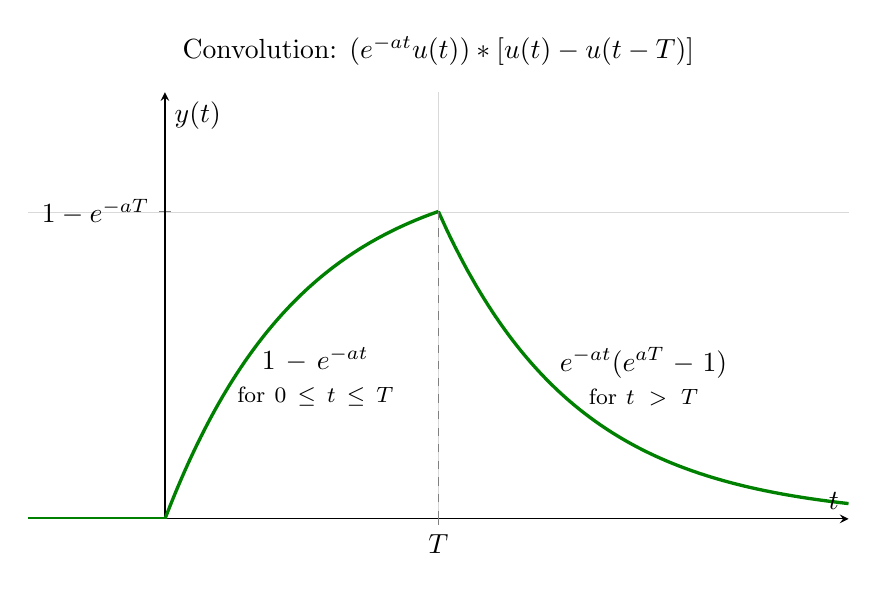
\begin{tikzpicture}
	\begin{axis}[
		width=12cm,
		height=7cm,
		title={Convolution: $(e^{-at}u(t)) * [u(t)-u(t-T)]$},
		xlabel={$t$},
		ylabel={$y(t)$},
		axis lines=middle,
		xmin=-1, xmax=5,
		ymin=0, ymax=1.2,
		xtick={2},
		xticklabels={$T$},
		ytick={0.864},
		yticklabels={$1-e^{-aT}$},
		grid=major,
		grid style={line width=.1pt, draw=gray!30},
		no marks,
		]
		
		% Plot the two parts of the convolution result for a=1, T=2
		\addplot[green!50!black, very thick, domain=0:2, samples=100] {1 - exp(-x)};
		\addplot[green!50!black, very thick, domain=2:5, samples=100] {exp(-x)*(exp(2)-1)};
		\draw[green!50!black, very thick] (axis cs:-1,0) -- (axis cs:0,0);
		
		% Add vertical line at t=T
		\draw[dashed, gray] (axis cs:2,0) -- (axis cs:2, {1-exp(-2)});
		
		% Add labels for the function segments
		\node[text width=3cm, align=center] at (axis cs:1.1, 0.4) {$1-e^{-at}$ \\ \footnotesize for $0 \le t \le T$};
		\node[text width=3cm, align=center] at (axis cs:3.5, 0.4) {$e^{-at}(e^{aT}-1)$ \\ \footnotesize for $t > T$};
		
	\end{axis}
\end{tikzpicture}